%% abtex2-modelo-projeto-pesquisa.tex, v-1.9.6 laurocesar
%% Copyright 2012-2016 by abnTeX2 group at http://www.abntex.net.br/ 
%%
%% This work may be distributed and/or modified under the
%% conditions of the LaTeX Project Public License, either version 1.3
%% of this license or (at your option) any later version.
%% The latest version of this license is in
%%   http://www.latex-project.org/lppl.txt
%% and version 1.3 or later is part of all distributions of LaTeX
%% version 2005/12/01 or later.
%%
%% This work has the LPPL maintenance status `maintained'.
%% 
%% The Current Maintainer of this work is the abnTeX2 team, led
%% by Lauro César Araujo. Further information are available on 
%% http://www.abntex.net.br/
%%
%% This work consists of the files abntex2-modelo-projeto-pesquisa.tex
%% and abntex2-modelo-references.bib
%%

% ------------------------------------------------------------------------
% ------------------------------------------------------------------------
% abnTeX2: Modelo de Projeto de pesquisa em conformidade com 
% ABNT NBR 15287:2011 Informação e documentação - Projeto de pesquisa -
% Apresentação 
% ------------------------------------------------------------------------ 
% ------------------------------------------------------------------------


\documentclass[
	% -- opções da classe memoir --
	12pt,				% tamanho da fonte
 	openright,			% capítulos começam em pág ímpar (insere página vazia caso preciso)
 	oneside,
 	%twoside,			% para impressão em recto e verso. Oposto a oneside
	a4paper,			% tamanho do papel. 
	% -- opções da classe abntex2 --
	%chapter=TITLE,		% títulos de capítulos convertidos em letras maiúsculas
	%section=TITLE,		% títulos de seções convertidos em letras maiúsculas
	%subsection=TITLE,	% títulos de subseções convertidos em letras maiúsculas
	%subsubsection=TITLE,% títulos de subsubseções convertidos em letras maiúsculas
	% -- opções do pacote babel --
	english,			% idioma adicional para hifenização
	french,				% idioma adicional para hifenização
	spanish,			% idioma adicional para hifenização
	brazil,				% o último idioma é o principal do documento
	]{abntex2}

% ---
% PACOTES
% ---

% ---
% Pacotes fundamentais 
% ---
\usepackage{lmodern}			% Usa a fonte Latin Modern
\usepackage[T1]{fontenc}		% Selecao de codigos de fonte.
\usepackage[utf8]{inputenc}		% Codificacao do documento (conversão automática dos acentos)
\usepackage{indentfirst}		% Indenta o primeiro parágrafo de cada seção.
\usepackage{color}				% Controle das cores
\usepackage{graphicx}			% Inclusão de gráficos
\usepackage{microtype} 			% para melhorias de justificação

% ---

% ---
% Pacotes adicionais, usados apenas no âmbito do Modelo Canônico do abnteX2
% ---
\usepackage{lipsum}				% para geração de dummy text
% ---

% ---
% Pacotes de citações
% ---
\usepackage[brazilian,hyperpageref]{backref}	 % Paginas com as citações na bibl
\usepackage[alf]{abntex2cite}	% Citações padrão ABNT

% --- 
% CONFIGURAÇÕES DE PACOTES
% --- 

% ---
% Configurações do pacote backref
% Usado sem a opção hyperpageref de backref
\renewcommand{\backrefpagesname}{Citado na(s) página(s):~}
% Texto padrão antes do número das páginas
\renewcommand{\backref}{}
% Define os textos da citação
\renewcommand*{\backrefalt}[4]{
	\ifcase #1 %
		Nenhuma citação no texto.%
	\or
		Citado na página #2.%
	\else
		Citado #1 vezes nas páginas #2.%
	\fi}%
% ---

% ---
% Informações de dados para CAPA e FOLHA DE ROSTO
% ---
\titulo{EducaLar - Aplicativo que conecta quem tem o conhecimento a quem precisa}
\autor{Caio Henrique Machado de Oliveira - 16101023 \\Karen Silva Santos - 16101845\\Lucas Góes - 16101762\\Lucas Magrini - 16100586\\Ricardo Aparecido Bezerra Elias da Silva - 15203158}
\local{Osasco}
\data{2018}
\instituicao{%
  Centro Universitário UNIFIEO
  \par
  Engenharia da Computação
  \par
  Engenharia de Software II}
\tipotrabalho{Tese (Doutorado)}
% O preambulo deve conter o tipo do trabalho, o objetivo, 
% o nome da instituição e a área de concentração 
\preambulo{Projeto de criação de um aplicativo mobile utilizando os conceitros de Engenharia de Software abordados em sala de aula.}
% ---

% ---
% Configurações de aparência do PDF final

% alterando o aspecto da cor azul
\definecolor{blue}{RGB}{41,5,195}

% informações do PDF
\makeatletter
\hypersetup{
     	%pagebackref=true,
		pdftitle={\@title}, 
		pdfauthor={\@author},
    	pdfsubject={\imprimirpreambulo},
	    pdfcreator={LaTeX with abnTeX2},
		pdfkeywords={abnt}{latex}{abntex}{abntex2}{projeto de pesquisa}, 
		colorlinks=true,       		% false: boxed links; true: colored links
    	linkcolor=blue,          	% color of internal links
    	citecolor=blue,        		% color of links to bibliography
    	filecolor=magenta,      		% color of file links
		urlcolor=blue,
		bookmarksdepth=4
}
\makeatother
% --- 

% --- 
% Espaçamentos entre linhas e parágrafos 
% --- 

% O tamanho do parágrafo é dado por:
\setlength{\parindent}{1.3cm}

% Controle do espaçamento entre um parágrafo e outro:
\setlength{\parskip}{0.2cm}  % tente também \onelineskip

% ---
% compila o indice
% ---
\makeindex
% ---

% ----
% Início do documento
% ----
\begin{document}

% Seleciona o idioma do documento (conforme pacotes do babel)
%\selectlanguage{english}
\selectlanguage{brazil}

% Retira espaço extra obsoleto entre as frases.
\frenchspacing 

% ----------------------------------------------------------
% ELEMENTOS PRÉ-TEXTUAIS
% ----------------------------------------------------------
% \pretextual

% ---
% Capa
% ---
\imprimircapa
\imprimirfolhaderosto

\pdfbookmark[0]{\contentsname}{toc}
\tableofcontents*
\cleardoublepage
% ---
\textual

% ----------------------------------------------------------
% Introdução
% ----------------------------------------------------------
\chapter[Justificativa]{Justificativa}

Com a massificação de celulares, uma grande quantidade de aplicativos \emph{mobile} é desenvolvida diariamente. Há de diversos tipos: produtividade, bem-estar, relacionamento, aprendizagem, vídeo, música, notícias, redes sociais, fotos, e mais uma imensidão de opções. 
Com isso é muito difícil encontrar uma pessoa que não possua um aplicativo que o auxilie em algo. 

Um dos aplicativos mais famosos, por exemplo, é o Tinder que possibilita o encontro de pessoas com interesses em comum, voltado a relacionamentos pessoais. O Tinder cruza algumas informações e apresenta opções ao usuário classificar se gostou ou não de determinada pessoa. Havendo uma resposta positiva (\emph{match}) e recíproca, essas duas pessoas podem estabelecer contato e então iniciar um relacionamento.

Outro aplicativo muito popular é o Uber, que permite ao usuário solicitar uma viagem pelo aplicativo onde o motorista é também um usuário que utiliza seu carro para executar a viagem. Estes aplicativos conectam dois lados de usuários que tem interesses em comum.

Pensando neste tipo de serviço identificamos que é possível disponibilizar uma plataforma em que pessoas que possuam bons conhecimentos em determinado assunto possam auxiliar outras que possuam dificuldades neste mesmo assunto, fornecendo assim um reforço educacional. 

Um exemplo de aplicação seria: um aluno do ensino médio possui dificuldades nas matérias de exatas e precisa de reforço para conseguir melhorar suas notas. Do outro lado há um estudante de letras que tem facilidade e dá aulas aos finais de semanas para seu primo. O aplicativo poderá unir estas duas pessoas em um bem comum.

% Separar em mais parágrafros
\chapter[Objetivos]{Objetivos}

% A priori, o objetivo era trazer educação para as pessoas que querem buscar conhecimentos para agregar em sua vida educacional ou para reforçar pontos que já foram vistos porém não totalmente compreendido. 

% Quando colocamos a tecnologia como um multiplicador percebemos que serviços de aulas online, por exemplo, já são amplamente oferecidos na internet e trazer outra plataforma de estudos para o mercado não daria um patamar para tal. Pensando nisso, surgiu a ideia de levar o educador ao educando possibilitando assim um estudo mais focado e direcionado.

Dar ao educador a possibilidade de disseminar seu conhecimento a quem necessita e dar ao educando a oportunidade de contar com uma pessoa que tenha tempo, localização e interesses compatíveis.

% Algumas partes podem ser direcionadas para justificativa
%\chapter[Conhecimento]{Conhecimento}

Para o desenvolvimento desta plataforma, entendemos ser necessário ter os seguintes conhecimentos:

\begin{alineas}
    \item Desenvolvimento Mobile:
        \par Este conhecimento auxiliará na criação do aplicativo e de recursos para que o software fique disponível para plataformas de celular.
    \item Design:
        \par Este conhecimento fornecerá usuário experiências amigáveis ao visualmente tornando a navegação no aplicativo fluente.
    \item Banco de Dados:
        \par Uma grande quantidade de dados será gerado e deve ser armazenado corretamente otimizando espaço e tempo de acesso.
    \item Redes e Servidores
        \par O aplicativa receberá diversos acessos pela rede e deverá estar disponível sempre que possível.
    \item Marketing
        \par Para divulgação do aplicativo nos canais de contato.
    \item Segurança da Informação
        \par Haverá dados de usuários, manter esses dados seguros deverão fazer parte do desenvolvimento.
\end{alineas}

% Pode ser diluída em Recursos e Equipe
\chapter[Recursos]{Recursos}

\section[Hardware]{Hardware}

\begin{alineas}
    \item 1x Switch para trafegar dados internamente.
    \item 1x Switch para trafegar dados externamente.
    \item 5x Computador Compaq Presario CQ14 Processador Intel® Core™ i3-6100T, Windows 10 Home, 4GB, HD 500GB, Gravador de DVD, HDMI.
    \item 10x Notbook HP 240G6 Core I5 Tela 14" 8GB 1TB Windows 10.
    \item 3x Tablets M7S Quad Core Android 4.4 Wi-FI 7 8GB Preto – Multilaser.
    \item 1x Servidor Dell PowerEdge T330 A20 E3-1220v6 8Gb 2x1Tb com Controladora.
    \item 1x Roteador D-Link DIR-878 Wireless AC Dual Band 1900 Mbps.
    \item 1x Servidor Power Edge T130.
    \item 13x Mouse Pad (Mouse Pad com apoio para punho Staples).
\end{alineas}

\section[Software]{Software}

\textit{Nota dos autores: Adicionar os softwares aqui. Quem está encarregado?}

% Colocar valores 
\chapter[Equipe]{Equipe}

Para a criação do aplicativo montaremos uma equipe com 12 pessoas, profissionais da área de tecnologia, que trabalharão em pequenas partes do desenvolvimento. O conjunto das partes resultará no EducaLar.


\begin{figure}[htb]
	%\caption{\label{gantt}Placa Wiring S}
	\begin{center}
	    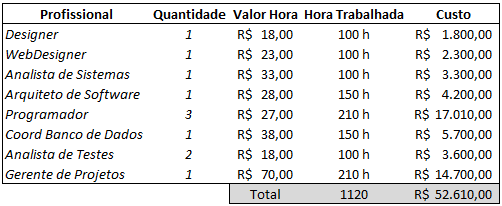
\includegraphics[scale=0.9]{tabelaCustos}
	\end{center}
	%\legend{Fonte: Site da 3GPP}
\end{figure}

%\begin{alineas}
%    \item Um Designer (ou \emph{Front End Designer}) %que é a pessoa %responsável por elaborar o desenho das interfaces do aplicativo.
%    \item Um Web designer %que vai ser responsável por aplicar o layout %projetado anteriormente.
%    \item Um Analista de sistemas %que vai ser responsável por %compreender a necessidade de negócio do cliente e especificar por %escrito o que precisa ser feito no projeto.
%    \item Um Arquiteto de software %que vai analisar as necessidades do %projeto e define a arquitetura técnica que melhor se encaixa no %projeto.
%    \item Cinco desenvolvedores/programadores %que vai transformar as %especificações de negócio do aplicativo em código sendo responsáveis %por 50 \% do esforço total do projeto de desenvolvimento e manutenção %do aplicativo.
%    \item Um analista de banco de dados %que vai tratar adequadamente %do grande volume de dados.
%    \item Um analista de testes %que vai fazer a validação do %aplicativo analisando todo sistema e vendo se não há erros %(\emph{bugs}) no aplicativo.
%    \item Gerente de projetos %que cria e acompanha o cronograma do %projeto, dando as diversas tarefas para os profissionais
%\end{alineas}
\chapter[Metas]{Metas}

%O projeto conta com quatro grandes metas principais, passando de criação e desenvolvimento até a parte de lançamento e estabilidade do aplicativo. 

%Como meta inicial, após a elaboração do plano de desenvolvimento do software, faremos a criação e desenvolvimento do aplicativo, parte principal do projeto, buscando robustez já na primeira versão.
% Está vago

%Como segundo passo, trazendo a tarefa que por muitos é dada como mais importante, fazer o teste do aplicativo que vai analisar os mínimos detalhes e possíveis falhas, possibilitando entregar uma versão o mais estável possível. 

%Fazer a divulgação por meio de feiras de ensino, escolas, nas diversas redes sociais e nos sites de ensino, buscando levar o aplicativo não só para as pessoas que querem aprender, mas sim, as que querem ensinar.

%Por último, a tarefa de manter o aplicativo no ar, trabalhando e assegurando que o aplicativo ficará 24 horas disponível e funcional.

% Separar em tópicos
% Aprofundar mais
% Alguns termos estão razos

\section[Cronograma]{Cronograma}

% Como estamos falando de um aplicativo de médio porte, padronizando horário com aplicativos criados ele demoraria de 500 a 800 horas para ser desenvolvido. 

A ideia sugere um aplicativo de médio porte, o que pode levar de 500 a 800 horas para ser desenvolvido, projetando um \textit{lead time} de 5 a 9 meses.

%---- Aqui vai uma tabela ----


\begin{table}[htb]
  \centering
  \caption[Cronograma]{Cronograma}
  \label{tabCrono}
  \begin{tabular}{llllllll}
    \textbf{Atividades} & \textbf{Jan} & \textbf{Fev} & \textbf{Mar} & \textbf{Abr} & \textbf{Mai} & \textbf{Jun} & \textbf{Jul} \\
    \hline
    Meta 1          & X   & X   & X   & X   & X   & X   & X   \\
    Meta 2  		& X   &     &     &     &     &     &     \\
    Meta 3      	& X   &     & X   &     & X   &     & X   \\
    Meta 4 	        &     & X   & X   &     &     &     &     \\
    Meta 5 	        &     & X   & X   & X   & X   & X   &     \\
    Meta 6 			&     & X   & X   & X   & X   & X   & X   \\
    Meta 7 			&     &     &     &     &     & X   & X   \\
    Meta 8 			&     &     &     &     &     & X   & X   \\
    Meta 9 			&     &     &     &     &     &     & X   \\
    Meta 10 		&     &     &     &     &     &     & X   \\
    \hline
  \end{tabular}
\end{table}


% Não está legal. Montar um cronograma \textit{like a} iniciação científica associando o tópico de metas


% Notas de Aula (CICLO DE VIDA)

% Prazos e Tarefas (Inicio, Desenvolvimento e Final) . Fase 1 discussão, planejamento, desenvolvimento planejamento.

% Cada etapa é uma tarefa. Cada tarefa tem um prazo. (HORAS)

%% CICLO
% Levantamento -> Análise - > Projeto -> Implementação -> Manutenção

% Requisito é etapa "Cada momento é um tempo, cada tempo é uma ação" (PROFESSORA)
\chapter[Cronograma]{Cronograma}


% Como estamos falando de um aplicativo de médio porte, padronizando horário com aplicativos criados ele demoraria de 500 a 800 horas para ser desenvolvido. 

O projeto levará 7 meses (1120 horas)

%---- Aqui vai uma tabela ----



\begin{figure}[htb]
	%\caption{\label{gantt}Placa Wiring S}
	\begin{center}
	    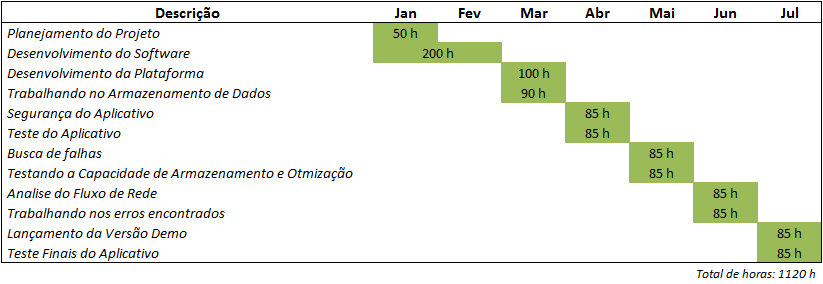
\includegraphics[scale=0.8]{diagramaGanttCrono}
	\end{center}
	%\legend{Fonte: Site da 3GPP}
\end{figure}


% Não está legal. Montar um cronograma \textit{like a} iniciação científica associando o tópico de metas


% Notas de Aula (CICLO DE VIDA)

% Prazos e Tarefas (Inicio, Desenvolvimento e Final) . Fase 1 discussão, planejamento, desenvolvimento planejamento.

% Cada etapa é uma tarefa. Cada tarefa tem um prazo. (HORAS)

%% CICLO
% Levantamento -> Análise - > Projeto -> Implementação -> Manutenção

% Requisito é etapa "Cada momento é um tempo, cada tempo é uma ação" (PROFESSORA)
\chapter[Investimento]{Investimento}

Para a realização deste projeto o valor do investimento será de 

% Novo tópico para divulgação?
%    \section[Divulgação]{Divulgação} 
%        Optaremos pela divulgação em redes socias, através de páginas gerenciadas pelos membros da equipe. Para uma penetração maior, optaremos por anúncios em apps de educação, gerando um custo estimado de R\$ 5 mil / ano.




%    \section[Manutenção e Mantenabilidade]{Manutenção e Mantenibilidade}
%        Barry Boehm propõe que o custo de manutenção de um software é de \$ 1 mil por linha de código. Além disso temos os custos de servidores de software que podem girar em torno de R\$ 20 mil / ano.


\chapter[Risco]{Risco}

Identificamos os seguintes riscos para execução do projeto:

\begin{alineas}
    \item Capital inferior ao necessário, tendo que recorrer a redução de custos deixando assim um padrão inferior ao desejado.
    \item Desistência do projeto devido a problemas financeiros.
    \item Problemas de gestão / operação.
    \item Atrasos na entrega das etapas.
    \item Problemas técnicos com aparelhos.
    \item Concorrência.
    \item Indisponibilidade de mercado para atuação.
\end{alineas}

% Professora quer mais detalhes em cada tópico


\phantompart
\postextual
\phantompart
\printindex

\end{document}
